% ---------------------------------------------------
%
% Trabajo de Fin de Grado. 
% Author: Laura Padrón Jorge. 
% Capítulo: Tecnologías utilizadas en el Trabajo de Fin de Grado. 
% Fichero: Cap2_Technology.tex
%
% ----------------------------------------------------
%

\cleardoublepage
\chapter{Herramientas y Tecnologías} \label{chap:Tecnologias} 

Este capítulo tiene como objetivo presentar las distintas herramientas software y tecnologías empleadas por la alumna en el desarrollo de \BulletPoint{}.

\section{Herramientas de Desarrollo}

A continuación se explicarán brevemente las distintas herramientas software utilizadas en el proyecto. 

\subsection{Android Studio}


\begin{itemize}
\item Un sistema de compilación basado en Gradle\cite{URL::Gradle} que ha simplificado tanto la inserción de dependencias de las distintas librerías que se han tenido que utilizar, como la compilación de la aplicación.
\item Un emulador rápido y fácil de utilizar que ha ayudado a visualizar las distintas pantallas durante el desarrollo aunque no ha sido de mucha utilidad para probar el funcionamiento al ser dependiente la app de la tecnología Bluetooth.
\item La facilidad para publicar cambios a aplicaciones ya funcionando sin tener que eliminar y volver a crear un nuevo APK parando la app.
\item Un sistema de visualización de las diferentes pantallas muy completo, con soporte visual para añadir componentes y cambiar atributos fácilmente.
\item Un sistema de depuración, con una interfaz sencilla e intuitiva.
\end{itemize} 

\begin{figure}[h]
	\centering
	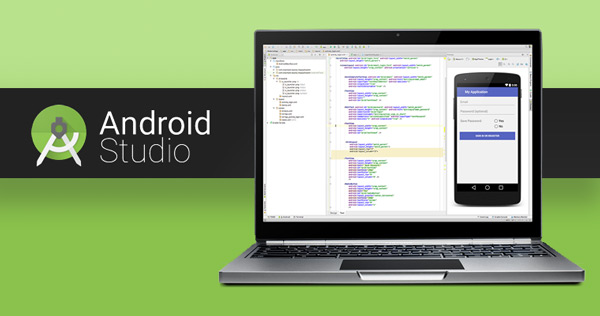
\includegraphics[width=0.6\linewidth]{androidstudio}
	\caption{Android Studio, un IDE flexible e intuitivo.}
	\label{fig:androidstudio}
\end{figure}

Se ha utilizado este IDE frente a otros como Eclipse + ADT \cite{URL::eclipseADT} debido a que en la actualidad es el IDE oficial con soporte de Google. Se ha preferido aprender a utilizar este entorno con vistas al futuro, ya que parece que se consolidará como el preferido para los desarrolladores Android.

Los \textit{``Beacons''} \cite{URL::Beacon} (la traducción del término sería a \textit{``balizas''} o \textit{``faros''}) son una tecnología emergente que desde hace algunos años intenta abrirse paso en el mercado. Como su propio nombre indica, estos dispositivos intentan ser un mecanismo de guía, dando una solución al posicionamiento en interiores, donde otras tecnologías, como el GPS \cite{URL::GPS} o el Wifi dejan de funcionar o resultan imprecisas. Sin embargo, estos no son los únicos usos de los beacons, actualmente muchas empresas están ampliando sus usos a otros campos.

